\usepackage{xcolor}
\usepackage{afterpage}
\usepackage{pifont,mdframed}
\usepackage[bottom]{footmisc}


\createsection{\Grader}{Sample grader}

\renewcommand{\inputfile}{\texttt{stdin}}
\renewcommand{\outputfile}{\texttt{stdout}}
\makeatletter
\renewcommand{\this@inputfilename}{\texttt{stdin}}
\renewcommand{\this@outputfilename}{\texttt{stdout}}
\makeatother

% % % % % % % % % % % % % % % % % % % % % % % % % % % % % % % % % % % % % % % % % % %
% % % % % % % % % % % % % % % % % % % % % % % % % % % % % % % % % % % % % % % % % % %

Cecilia is the most ``environmentalist'' team member in the OII, always
attentive to respecting nature and sorting the trash. Naturally, she has a
garden at home: a long, straight patch of soil, in which she planted $N$ seeds.
Each seed was planted at a specific distance $X_i$ from the start of the garden
and at a specific depth $P_i$. All these values are expressed in millimeters:
the seeds are, however, always planted in positions that are multiple of $1$cm
for technical reasons (i.e. $X_i$ and $P_i$ are always divisible by $10$).

To wet her seeds, Cecilia is going to install some sprinklers along the surface
of her garden. These will spray water that, because of the soil's permeability,
will reach the deep buried seeds. When a sprinkler is turned on, the sprayed
water will spread along the surface with a speed of $1$ millimeter per second
both to the right and to the left. Each point, after becoming wet, will start
expanding downwards into the soil at the same speed. This will form a
triangle-shaped wet soil area:%
%
\begin{figure}[H]
  \centering
  \includegraphics[width=.78\linewidth]{asy_orticoltura/fig0.pdf}
  \caption{Two sprinklers located at $38$mm and $70$mm, turned on for $26$ and $20$ seconds respectively.}
\end{figure}

For example, in Figure 1 the two rightmost seeds are wet, but the leftmost seed
is still dry. Notice that different sprinklers do not influence each other. More
specifically, if we identify with $(X_{seed}, P_{seed})$ some seed's
coordinates, with $X_{sprinkler}$ the position of a sprinkler and with
$T_{sprinkler}$ its sprinkle duration, we can say that a seed is wet if:

$$|X_{seed}-X_{sprinkler}| + P_{seed} \le T_{sprinkler}$$

Cecilia will sustain a fixed cost and a variable cost for each sprinkler. Buying
a sprinkler is $C$ euro cents, and using it costs $1$ cent per second. The
sprinklers can be scheduled to be on for different amounts of time, but the time
must always be a multiple of $1$ second. Moreover, each sprinkler must be
installed at a distance from the start of the garden that is multiple of $1$mm.

Help Cecilia buy, install and schedule the sprinklers so that all the seeds will
be wet, while minimizing the total cost of the garden!

% % % % % % % % % % % % % % % % % % % % % % % % % % % % % % % % % % % % % % % % % % %
% % % % % % % % % % % % % % % % % % % % % % % % % % % % % % % % % % % % % % % % % % %


\Implementation

You should submit a single file, with either a \texttt{.c} or \texttt{.cpp}
extension.

\begin{warning}
Among the attachments in this task you will find a template
\texttt{orticoltura.c} or \texttt{orticoltura.cpp} with a sample implementation.
\end{warning}

You will have to implement the following function:

\begin{center}\begin{tabularx}{\textwidth}{|c|X|}
\hline
C    & \verb|void irriga(int C, int N, int* X, int* P);|\\
C++  & \verb|void irriga(int C, int N, vector<int>& X, vector<int>& P);|\\
\hline
\end{tabularx}\end{center}

\begin{itemize}[nolistsep]
  \item The integer $C$ is the fixed cost for each sprinkler installed.
  \item The integer $N$ is the number of seeds planted in the garden.
  \item The array \texttt{X}, indexed from $0$ to $N-1$, contains the list of seeds' positions.
  \item The array \texttt{P}, indexed from $0$ to $N-1$, contains the list of seeds' depths.
\end{itemize}

\medskip

Your program can use the following functions, which are already defined in the
grader:

\begin{center}\begin{tabularx}{\textwidth}{|c|X|}
\hline
C/C++  & \verb|void posiziona(int D, int T);|\\
\hline
\end{tabularx}\end{center}

\begin{itemize}[nolistsep]
  \item The integer $D > 0$ is the position where to install a sprinkler.
  \item The integer $T > 0$ is how long the sprinkler will be on for.
\end{itemize}

\medskip

\begin{center}\begin{tabularx}{\textwidth}{|c|X|}
\hline
C/C++  & \verb|void budget(int B);|\\
\hline
\end{tabularx}\end{center}

\begin{itemize}[nolistsep]
  \item The integer $B$ is the minimum total cost that Cecilia should pay to wet
  all her seeds.
\end{itemize}

\medskip

The grader will call the \texttt{irriga} function. From there, you will be able
to call the function \verb|posiziona| to install new sprinklers or call the
\verb|budget| function to return the total minimum cost to be paid. The order in
which you will call the \verb|posiziona| function is not important. In case of
multiple calls to the \verb|budget| function only the last one will be
considered.

% % % % % % % % % % % % % % % % % % % % % % % % % % % % % % % % % % % % % % % % % % %
% % % % % % % % % % % % % % % % % % % % % % % % % % % % % % % % % % % % % % % % % % %

\Grader

Among this task's attachments you will find a simplified version of the grader
used during evaluation, which you can use to test your solutions locally. The
sample grader reads data from \inputfile{}, calls the functions that you should
implement and writes back on \outputfile{} using the following format.

The input file is formed by $N+1$ lines:
\begin{itemize}[nolistsep,itemsep=2mm]
\item Line $1$: the integer $C$, the cost of a sprinkler.
\item Line $2$: the integer $N$, the number of seeds.
\item Lines $3\ldots N+2$: the values of \texttt{X[$i$]} and \texttt{P[$i$]} for
$i = 0\ldots N-1$.
\end{itemize}

The output file is formed by $K+2$ lines:
\begin{itemize}[nolistsep,itemsep=2mm]
\item Line $1$: the integer $B$, the total cost found for the sprinklers.
\item Line $2$: the integer $K$, the number of sprinklers used.
\item Lines $3\ldots K+2$: the values of \texttt{D[$j$]} and \texttt{T[$j$]} for
$j = 0\ldots K-1$.
\end{itemize}

% % % % % % % % % % % % % % % % % % % % % % % % % % % % % % % % % % % % % % % % % % %
% % % % % % % % % % % % % % % % % % % % % % % % % % % % % % % % % % % % % % % % % % %


\Constraints

\begin{itemize}[nolistsep, itemsep=2mm]
	\item $0 \le C \le 10^9$.
	\item $1 \le N \le 1\,000\,000$.
	\item $10 \le X_i, P_i \le 10^9$ and they're multiples of $10$, for each
	$i=0\ldots N-1$.
	\item There are no two seeds at the same position and depth.
\end{itemize}

% % % % % % % % % % % % % % % % % % % % % % % % % % % % % % % % % % % % % % % % % % %
% % % % % % % % % % % % % % % % % % % % % % % % % % % % % % % % % % % % % % % % % % %

\pagebreak

\Scoring

Your program will be tested on a number of testcases grouped in subtasks. For
each test case, the score is divided in two parts:

\begin{itemize}[nolistsep,itemsep=2mm]
  \item $60\%$ of the score: if the cost returned by \verb|budget| is the minimum cost to wet all seeds;
  \item $40\%$ of the score: if the calls to \verb|posiziona| install the sprinklers in an optimal way.
\end{itemize}

The score for a subtask is given by the total points of the subtask, multiplied
by the \textbf{minimum} score obtained on any of its testcases.

\begin{itemize}[nolistsep,itemsep=2mm]
  \item \textbf{\makebox[2cm][l]{Subtask 1} [\phantom{0}0 points]}: Sample testcases.
  % esponenziale becera
  \item \textbf{\makebox[2cm][l]{Subtask 2} [\phantom{0}5 points]}: $N \leq 4$, $X_i \leq 100$, $P_i = 10$.
  % dinamica O(N²) senza profondità
  \item \textbf{\makebox[2cm][l]{Subtask 3} [15 points]}: $N \leq 1000$ e $P_i = 10$.
  % nessun problema di arrotondamento
  \item \textbf{\makebox[2cm][l]{Subtask 4} [20 points]}: $P_i = 10$.
  % dinamica O(N²)
  \item \textbf{\makebox[2cm][l]{Subtask 5} [20 points]}: $N \leq 1000$.
  % merge dei triangoli
  \item \textbf{\makebox[2cm][l]{Subtask 6} [20 points]}: $C = 0$.
  % merge dei triangoli + traslazione / dinamica / greedy sortando per X-P
  \item \textbf{\makebox[2cm][l]{Subtask 7} [20 points]}: No limits.
\end{itemize}

% % % % % % % % % % % % % % % % % % % % % % % % % % % % % % % % % % % % % % % % % % %
% % % % % % % % % % % % % % % % % % % % % % % % % % % % % % % % % % % % % % % % % % %


\Examples

\begin{example}
\exmpfile{orticoltura.input0.txt}{orticoltura.output0.txt}%
\exmpfile{orticoltura.input1.txt}{orticoltura.output1.txt}%
\end{example}

% % % % % % % % % % % % % % % % % % % % % % % % % % % % % % % % % % % % % % % % % % %
% % % % % % % % % % % % % % % % % % % % % % % % % % % % % % % % % % % % % % % % % % %


\Explanation

In the \textbf{first sample testcase}, this is a possible solution: \\[-22pt]
%
\begin{center}
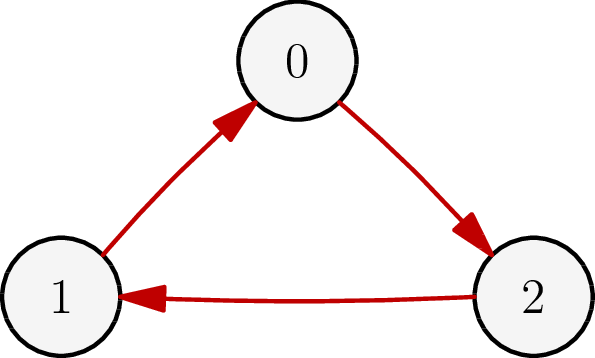
\includegraphics[width=.8\linewidth]{asy_orticoltura/fig1.pdf}
\end{center}

In the \textbf{second sample testcase}, this is a possible solution:
%
\begin{center}
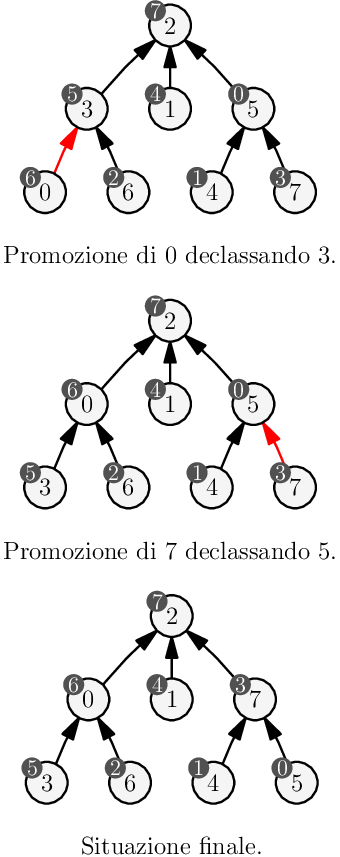
\includegraphics[width=.8\linewidth]{asy_orticoltura/fig2.pdf}
\end{center}
